\documentclass[11pt,letterpaper]{article}
\usepackage[utf8]{inputenc}
\usepackage{graphicx, geometry, amsmath, hyperref, url, natbib, booktabs, longtable, xcolor, array}
\geometry{margin=1in}
\setlength{\tabcolsep}{4pt}
\sloppy
\hypersetup{colorlinks=true, linkcolor=black, citecolor=black, urlcolor=black}
\renewcommand{\topfraction}{0.9}
\renewcommand{\bottomfraction}{0.8}
\renewcommand{\textfraction}{0.07}
\renewcommand{\floatpagefraction}{0.75}

\title{Barometric formulas and the boiling point of water with altitude:\\internal research report}
\author{Internal research record}
\date{\today}

\begin{document}
\maketitle
\tableofcontents

\section{Question and framing}

This run asks how well a simple barometric formula predicts the boiling point of water at altitude, compared with published measurements. The hypothesis couples a barometric pressure-altitude formula to the saturation vapour pressure curve of water, using the Wagner and Pru\ss{} formulation [1]. It predicts that the calculated boiling temperature matches measured values to about $\pm 0.3$\,$^\circ$C from sea level to 4,000 m when station pressure is used, and to about $\pm 0.6$\,$^\circ$C when only altitude is known and standard-atmosphere pressure is assumed. It also predicts that most of the residual comes from weather-driven pressure deviations, and that the structural difference between the isothermal and the lapse-rate barometric forms is about 0.3\,K at 3,000 m and 0.5\,K at 4,000 m.

Two quantities recur in this document, and each is defined once here. The \emph{structural term} at an altitude $z$ is the boiling temperature given by the isothermal barometric form minus the boiling temperature given by the lapse-rate form at the same $z$, both converted with the same saturation curve. The \emph{total error budget} of 0.6\,K is the bound the hypothesis sets on predicted minus measured boiling temperature. The structural term is a property of the two formulas and the reference atmosphere. It is not a measured residual, and it cannot be tested against the 0.6\,K bound on its own.

Testing the claim needs three things: measured boiling records with paired station pressure and elevation, a saturation curve, and the barometric chain that connects them. The run tried to collect the first and did not succeed. Its evidence is therefore a model-to-reference screen of the physics chain, together with reference tables that were calculated rather than measured. The measured comparison that the hypothesis asks for has not been run. The sections below record each iteration in the order it ran, with its artifacts, its numbers, the reviewer's objections and the hypothesis update that followed.

\section{Iteration 1}

\subsection{Strategy and the reasoning behind it}

Iteration 1 was the first iteration, so no earlier review existed to answer. The strategy had three aims, in this order:
\begin{enumerate}
\item Collect published site records (elevation, station pressure, observed boiling temperature), so that predicted and observed boiling points could be compared directly.
\item Screen the barometric formulas against a reference pressure model and the water saturation curve, so that the size of the structural term is known before weather is added.
\item Screen cheaper closed-form alternatives (constant and temperature-dependent latent heat Clausius--Clapeyron, and an Antoine equation) against the same reference curve, because these are the shortcuts a practitioner would use.
\end{enumerate}

The planning record states the selection rule before any screen ran. A candidate survives if its maximum absolute error against the reference is at or below 0.6\,$^\circ$C anywhere from 0 to 4,000 m. Survivors are ranked by root-mean-square (RMS) error over that grid. The planner expected the isothermal-minus-lapse-rate structural term to be near 0.6\,K at 4,000 m by a rough estimate, which is above the hypothesis's 0.5\,K, and it stated that the experiment must report the measured number rather than a threshold adjusted to fit it.

The plan named four candidate methods for the altitude-to-boiling-point map: the barometric chain, the closed-form vapour-pressure routes, an empirical altitude fit, and a local pressure calibration from weather records. Only the first two could be tested against a reference in this iteration. The empirical fit and the local calibration were recorded as candidates that need measured sites first, and no artifact for either was run. The expected outcome was a ranked comparison on one shared reference grid and a sourced dataset of at least 25 published boiling-point records, with one third held out for later confirmation. The first aim failed, as the next subsection records.

\subsection{Artifacts run in iteration 1}

\subsubsection{Reference table of boiling temperature against elevation}

This dataset is a 41-row table of boiling temperature from 0 to 4,000 m, in 100 m steps. Each row is labelled \texttt{equation\_derived} in its own metadata. The table was built so that a later step could add measured sites under the same schema, with a predefined holdout rule (measured sites in the Americas above 1,000 m). No measured site was added, so the measured-site count is zero and the holdout set is empty. No measured rows were padded in from calculated values.

\emph{Correction recorded in iteration 2:} the first wording of this section described each row as calculated from a published equation. That wording is withdrawn. The boiling values were copied from a boiling-temperature-by-elevation table on a public web page (deleze.name, accessed 21 November 2026). The artifact labels the rows as equation-derived because of the kind of table, not because the run verified a derivation. The provenance is therefore a web table of unverified origin, and the reader should treat its agreement with the formula check as an agreement between two calculations.

The artifact also carries a formula check. It compares each row with an altitude-to-boiling-point calculation built from the U.S. Standard Atmosphere 1976 troposphere pressure and an empirical pressure-to-boiling-point fit. The residual column in the artifact's file is formula minus table, and Table~\ref{tab:ref-table} gives all 41 rows with that sign. Its mean is $-0.004390$\,$^\circ$C and its largest absolute value is 0.21\,$^\circ$C. The residuals in the earlier draft of this section had the opposite sign convention and were recomputed from the file for this report. The agreement shows that the two calculations are consistent with each other. It does not test the barometric chain against measurements.

\input{tables/tab_ref_table.tex}

\subsubsection{Reference-grid screen of the barometric forms}

The artifact gen\_art\_experiment\_1 ran this screen. It was built to compute, on one grid from 0 to 4,000 m, the boiling temperature implied by each barometric form, and to check the saturation inversion and the reference pressures before the structural term was read off. It wrote a 41-row grid file (results/grid\_values.csv, Table~\ref{tab:grid-structural}), a summary of its error statistics and verdicts (results/summary.json), and a method output file (method\_out.json) in the same format as the other artifacts. Its eleven recorded tests are listed in Table~\ref{tab:exp1-checks}, and all eleven pass. They cover the saturation inversion, the monotonicity of each form, the sea-level consistency, the structural-term size and the iapws cross-check. The isothermal-form verdict on the 0.6\,K bound is recorded separately as ``borderline: no pass/fail claim'', and that verdict is not one of the eleven tests.

This experiment asks how far the isothermal barometric formula departs from the standard lapse-rate form once each is converted to a boiling temperature with the water saturation curve. The isothermal form uses one scale height, which is $8{,}434.5$\,m (from $RT/Mg$ at 288.15 K). The lapse-rate form uses $L = 6.5$\,K/km. The lapse-rate form is also the reference pressure model, so its own error is zero by construction. The only informative error is the isothermal form measured against that reference. The structural term is the difference between the two boiling temperatures.

The saturation curve is the Wagner and Pru\ss{} formulation [1], inverted by bisection. Its checks passed. The boiling temperature at 101,325\,Pa is 373.1243\,K (99.9743\,$^\circ$C). The round-trip relative error of the saturation pressure at the inverted temperature is $4.22 \times 10^{-15}$. A separate calculation with the \texttt{iapws} package reproduces the sea-level and the 0, 2,000 and 4,000 m values to within 0.00024\,K.

\emph{Correction recorded in iteration 2:} the lapse-rate pressures were compared with standard-atmosphere node values that were typed in from a table recalled while the run was built, not read from the primary source. The 0.0073\,\% agreement therefore checks the formula against remembered values. It is not a verification of the reference against the document. The primary standard-atmosphere document was not read in either iteration.

The experiment's summary gives the error statistics against the reference. The isothermal form has a maximum absolute error of 0.588101\,K at 4,000 m and an RMS error of 0.268641\,K over the grid. The structural term is 0.332247\,K at 3,000 m, close to the hypothesis's 0.3\,K. At 4,000 m it is 0.588101\,K, above the hypothesis's ``about 0.5\,$^\circ$C'' and above the 0.5\,K structural target. The experiment's own verdict on the 0.6\,K bound was labelled borderline, with a margin of 0.011899\,K. The experiment made no pass or fail claim.

\emph{Correction recorded in iteration 2:} the 0.6\,K limit applies to total predicted-minus-measured error, which includes measurement and weather error. The structural term is a model-structure budget and cannot be tested against that limit. The ``borderline'' framing of the structural term is withdrawn. The term is tested against the 0.5\,K structural target, which it misses at 4,000 m. The 0.6\,K total bound remains untested until measured residuals exist.

Table~\ref{tab:grid-structural} gives all 41 grid rows, and Figure~\ref{fig:structural} plots the structural term against altitude. The line in that figure joins the 500 m nodes and is not a fit. An earlier draft described the rise as roughly the square of altitude, from a visual reading of the table. No fit was run, so that description is not used here.

\input{tables/tab_grid_structural.tex}

\input{tables/tab_exp1_checks.tex}

\begin{figure}[!htbp]
  \centering
  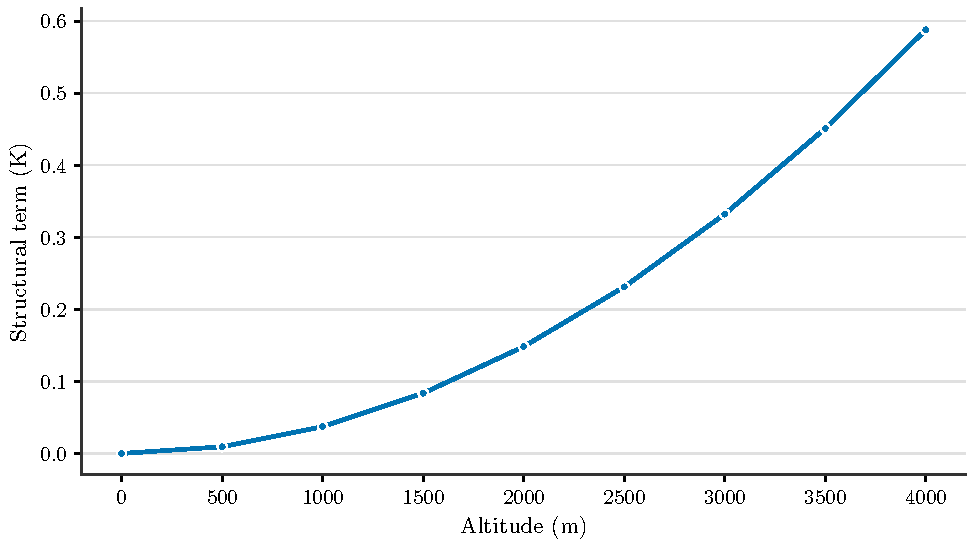
\includegraphics[width=\linewidth,height=0.45\textheight,keepaspectratio]{figures/fig1_v0.pdf}
  \caption{Structural term (isothermal minus lapse-rate boiling temperature, K) against altitude from 0 to 4,000 m, at the nine 500 m nodes of the reference-grid experiment (markers). The line joins the nodes and is not a fit. It is a model-structure term against the standard-atmosphere reference, not a comparison with measured boiling points.}
  \label{fig:structural}
\end{figure}

\subsubsection{Closed-form routes against the IAPWS-IF97 saturation curve}

The artifact gen\_art\_experiment\_2 ran this screen. It was built to compare the three closed-form routes with the IAPWS-IF97 curve over the same grid, to refit the Antoine constants, and to run a set of reference checks before the route errors were trusted. Its output files are: a summary table of route errors (results/summary.md, Table~\ref{tab:closed-form-iter1}); the refitted Antoine constants and fit residuals (results/antoine\_fit.json, Table~\ref{tab:antoine-fits}); the reference checks (results/reference\_checks.json, Table~\ref{tab:exp2-refchecks}); the independent recomputation at three altitudes (results/rederivation.json, Table~\ref{tab:exp2-points}); and two lookup and configuration files, results/lv\_table.json and results/method\_grid.json. The two lookup files are inputs to the screen, not result tables. results/lv\_table.json holds 201 temperatures from 273.15 K with the latent heat at each, and the grid mean of that latent heat, which route (b) and the sensitivity case use. results/method\_grid.json holds the grid, the anchor, the survival rule and the ranking rule. The run log is in results/run\_log.txt. Of the six reference-check entries in Table~\ref{tab:exp2-refchecks}, four pass, the Clapeyron check fails at its 1\,\% tolerance, and the anchor-identity entry carries no verdict.

This experiment screens three closed-form routes for the boiling temperature against the IAPWS Industrial Formulation 1997 saturation curve, region 4, through the \texttt{iapws} package. The three routes are:
\begin{itemize}
\item (a) Clausius--Clapeyron with a constant latent heat, anchored at the normal boiling point (373.124\,K). This is the textbook route and the primary method.
\item (b) Clausius--Clapeyron with a temperature-dependent latent heat, integrated from the same anchor with enthalpies from IAPWS-IF97.
\item (c) The Antoine equation, with constants refitted to the reference over 273.15 to 373.15 K. The starting constants came from the NIST WebBook water entry.
\end{itemize}
Each route is inverted for temperature on an 81-point grid from 0 to 4,000 m in 50 m steps. Pressure comes from the U.S. Standard Atmosphere 1976 troposphere formula. A sensitivity case with the grid-mean latent heat is reported but not ranked.

Table~\ref{tab:closed-form-iter1} gives the errors. The refitted Antoine equation has the smallest error of the three. Its largest error, 0.0042\,K, is at sea level. The constant-latent-heat form has errors that grow with altitude to 0.2780\,K at 4,000 m. Using the grid-mean latent heat instead of the anchored value makes the error 0.4069\,K at 4,000 m, which shows how sensitive the constant-latent-heat route is to the choice of that one constant. The experiment ranks the routes by RMS: Antoine (0.0022\,K), temperature-dependent latent heat (0.1082\,K), constant latent heat (0.1521\,K).

\emph{Correction recorded in iteration 2:} the Antoine row and the ranking are in-sample. The constants were refitted to the same IAPWS-IF97 reference over 273.15 to 373.15 K, and that reference then scored the method over 0 to 4,000 m. The 0.0042\,K figure is a fit-quality statement, not a predictive error. The same experiment's own fit residual over the full fit range was RMS 0.055289\,K and maximum 0.192233\,K after inversion (Table~\ref{tab:antoine-fits}), which Table~\ref{tab:closed-form-iter1} does not show. The earlier sentence that the refitted Antoine equation ``stays within 0.004\,K of the saturation curve over the grid'' is withdrawn for the same reason. The two figures come from different sets of points, so they should be read side by side and not as one error.

\input{tables/tab_closed_form_iter1.tex}
\input{tables/tab_antoine_fits.tex}
\input{tables/tab_exp2_refchecks.tex}
\input{tables/tab_exp2_points.tex}

The experiment's consistency check of the Clapeyron relation at a 1\,\% tolerance failed, with a maximum deviation of 1.59\,\% and a median of 0.52\,\%. The experiment attributed the deviation to the ideal-vapour factor, the compressibility of the vapour, $1/Z_\mathrm{v}$, which is about 1.6\,\% at 373 K. In iteration 1 this was the artifact's expectation written into its interpretation, not a tested result. Iteration 2 tested it directly. The check was reported as failed and was not corrected or relaxed.

\subsection{Review after iteration 1}

The reviewer gave iteration 1 a review score of 3, not blocking. The reviewer recomputed the reference table residuals, the structural term and the route statistics from their files, and found them to match. The reviewer's main objections were these.
\begin{itemize}
\item \textbf{Scope (major).} The request asks how well the barometric formula predicts measured boiling points. The run had zero measured sites, so that comparison was never made. The report answered a neighbouring question, the size of the structural term against the reference.
\item \textbf{Evidence (major).} The statement that Antoine stays within 0.004\,K omitted the fit-range inversion residual that the experiment reports.
\item \textbf{Rigour (major).} The Antoine refit was scored in-sample against the reference it was fitted to, so ranking it first was a fit-quality result, not a method comparison. A held-out split was requested.
\item \textbf{Evidence (major).} The reference table's provenance was misstated as an equation, and its web source was not named.
\item \textbf{Novelty (major).} Positive claims were made without naming the nearest published result, and no scholarly search was run.
\item \textbf{Rigour (major).} The 0.6\,K bound was applied to a structural term, and the verdict pulled against the 0.5\,K target.
\item \textbf{Rigour (minor).} The standard-atmosphere node values were recalled, not read from a source, so the 0.0073\,\% agreement is not a verification.
\item \textbf{Rigour (minor).} The 1/Z$_\mathrm{v}$ attribution of the Clapeyron failure was an expectation, not a test.
\item \textbf{Clarity (minor).} Two recomputation scripts were run but not described. The square-of-altitude wording was a visual reading. The log path discrepancy between storage volumes was disclosed but not resolved.
\end{itemize}

The reviewer's suggested actions became the work plan of iteration 2. Iteration 2 took the measured-record search first, the held-out Antoine split second, and the test of the Clapeyron attribution third.

\subsection{Hypothesis update after iteration 1}

The update was a \emph{cover} move. Only the measured comparison was open, and the reference screens cannot test the 0.3\,K or 0.6\,K claims. The update recorded that the 4,000 m structural term of 0.588\,K contradicts the 0.5\,K target, and that the 3,000 m value of 0.332\,K is near its 0.3\,K target. The 0.6\,K bound was kept as a total-error claim, untested until measured residuals exist. The alternative claim that variable latent heat more than halves the error was not supported: the executed values, 0.177\,K against 0.278\,K, are a reduction of about 36\,\%. The Antoine ranking was marked in-sample. The evidence state was graded weak or null, and the confidence in the hypothesis decreased.

\subsection{Dead ends in iteration 1}

\begin{itemize}
\item \textbf{Measured site records: not obtained.} Three candidate publications with site-level boiling records could not be read, because the publisher page or the journal full text returned HTTP 403. No site was verified, and the measured comparison was not run. The measured-site count is zero and the holdout set is empty.
\item \textbf{Weather-driven pressure deviation: not tested.} No station pressure series was used, so the claim that most of the residual comes from weather could not be assessed.
\item \textbf{Clapeyron consistency at 1\,\%: failed.} The failure was reported as a failure. Its attribution was untested at the time.
\item \textbf{Primary source for the standard atmosphere: not read.} The lapse rate, the sea-level values and the troposphere extent came from a secondary summary, because the primary PDF exceeded the fetch size limit.
\item \textbf{Log path discrepancy.} The run log of the grid experiment records its output paths on a different storage volume from the one the artifact sits on. The result files were read for every number in this document.
\end{itemize}

\subsection{Result of iteration 1}

On the reference equations alone, a constant-lapse-rate barometric formula and an isothermal one differ by a structural term of 0.332\,K at 3,000 m and 0.588\,K at 4,000 m. The isothermal form's maximum error against the reference is 0.588101\,K at 4,000 m. The anchored constant-latent-heat Clausius--Clapeyron route reaches 0.2780\,K at 4,000 m. The refitted Antoine equation's in-sample figures are reported above, with the fit-range residual that the reviewer asked for. These numbers describe the size of the model-structure term. They do not describe how well the chain agrees with measured boiling points, which was the hypothesis's question.

\subsection{Closing summary of iteration 1, as written at the time}

The summary below is kept as the record of what was believed at the end of iteration 1. Two of its statements were later corrected, as the sections above record: the 0.004\,K Antoine figure, and the description of the reference table as calculated from an equation.

\begin{itemize}
\item The structural term of the isothermal barometric form is 0.33\,K at 3,000 m and 0.59\,K at 4,000 m, against the hypothesis's predicted 0.3\,K and about 0.5\,K. The 4,000 m value exceeds the stated target.
\item The refitted Antoine equation reproduces the water saturation curve to 0.004\,K over 0 to 4,000 m, and the anchored constant-latent-heat Clausius--Clapeyron route reaches 0.28\,K at 4,000 m. \emph{[Corrected in iteration 2.]}
\item The published reference table and its formula check agree with each other to 0.21\,K at most, but that agreement is between two calculations, and no measured record has been compared with either.
\item The measured comparison, the weather-driven pressure deviation and the test of the $\pm 0.3$\,$^\circ$C and $\pm 0.6$\,$^\circ$C predictions have not been run.
\end{itemize}

\section{Iteration 2}

\subsection{Strategy and why this iteration ran what it ran}

Iteration 2 answered the reviewer's principal objection, which was that the run had answered a neighbouring question. The measured comparison was still open, and every other objection was a defect in the record of iteration 1. The strategy had three slots, and the plan fixed its decision rule before any analysis ran. The plan stated that if fewer than 15 sites with reliable inputs could be verified, the residual test would be reported as underpowered and the 0.3\,$^\circ$C and 0.6\,$^\circ$C claims would stay untested, not reshaped to fit.

\begin{enumerate}
\item A search for measured boiling records with paired station pressure and elevation (gen\_art\_dataset\_2). The target was at least 25 measured sites, with a fixed holdout of at least eight. It was the first thing the strategy asked for, and its result decides what the rest of the iteration can say.
\item A test of the isothermal and lapse-rate chain against those records (gen\_art\_experiment\_3), built to run the hypothesis's residual, structural-term and weather-term decomposition as soon as sites were accepted. It was written to report underpowered rather than a verdict when the accepted set was smaller than its minimum.
\item A re-screen of the three closed-form routes with a held-out split of the Antoine fit, a Z$_\mathrm{v}$-corrected Clapeyron check and an independent IAPWS-95 check (gen\_art\_experiment\_4). It answers the in-sample objection and the attribution objection.
\end{enumerate}

Of the sources the reviewer named, NOAA GHCN-Daily station pressure and the NIST steam-table PDF were on the planned list. The search did not reach them, as the dead-end list below records.

\subsection{Artifacts run in iteration 2}

\subsubsection{Search for measured boiling-point records}

The search covered eight broad web queries, page fetches of the most promising leads, and a Hugging Face search. No record meeting all four measured-record criteria (station pressure, elevation, observed boiling temperature and thermometer uncertainty) was verified. The best lead was Forbes (1857), which reports 17 boiling-point and barometer pairs at Alpine stations. Its table is damaged by optical character recognition in the archive text, and the site elevations are not in the copies the run could read, so no row passed the drop rules. The Denver Public Library index card was dropped because it has no date and no thermometer uncertainty. The Snyder calibration tables and the NBS steam tables are calculated rather than measured, and they were kept only as reference values.

Table~\ref{tab:candidates} gives the candidate log of the test artifact, which screened six sources and recorded the reason each was dropped. The sources are listed after the table.

\input{tables/tab_candidates.tex}
\input{tables/cand_urls.tex}

Table~\ref{tab:tierC} gives the only rows in the search dataset. They are the four Snyder reference values, converted from the source's Fahrenheit values. Each is labelled Tier C, which means equation-derived or handbook reference, and none is a measurement. The dataset's metadata records zero measured rows.

\input{tables/tab_tierC.tex}

\emph{Result of gen\_art\_dataset\_2: zero measured rows.} The measured-site count and the holdout are both empty, the same state as iteration 1.

\subsubsection{Test of the barometric chain against measured records}

This experiment was built to run the full chain once records exist. It inverts the Wagner and Pru\ss{} (IAPWS-95) saturation equation by bisection [1], with checks at the normal boiling point, the triple point and a round-trip inversion. Those checks pass, with a round-trip error of $3.7 \times 10^{-10}$\,K and a cross-check against the \texttt{iapws} package (IAPWS-IF97 region 4) at a maximum difference of 0.0019570\,K. The experiment computes residuals of the isothermal and lapse-rate forms, the structural term, the weather term (lapse-rate method minus measured pressure), bootstrap intervals over sites with a fixed seed, and a verdict for each claim. It requires at least 15 accepted sites, and it uses a holdout fixed in advance: every third site after sorting by elevation.

The accepted set is empty. Every claim is therefore marked ``UNDERPOWERED: untested'', and the residual statistics for both the full set and the holdout are recorded as $n = 0$ with no values. The bootstrap is recorded as ``no sites''. The only numbers the artifact produced are the model-only reference-grid structural term. Table~\ref{tab:claims} gives the verdicts, and Table~\ref{tab:struct-nodes} gives the structural term at the 500 m nodes from both iterations.

The artifact's output file names the three claims by letter and gives their verdicts, but it does not spell out the wording of each claim. This document therefore does not map the claims onto the hypothesis's criteria. Whatever the mapping, all three verdicts are untested, because no site was accepted.

\input{tables/tab_claims.tex}
\input{tables/tab_struct_nodes.tex}

The structural term reproduces the iteration 1 values to within $10^{-5}$\,K at every altitude. That agreement shows that the two runs reproduce each other. It says nothing about measured residuals. The artifact labels its own figure ``model-only reference-grid structural term; not validation''.

\emph{Result of gen\_art\_experiment\_3: no measured residual, weather term or holdout statistic was computed.} The structural term is reproduced, and the 4,000 m value of 0.588092\,K is 0.088092\,K above the 0.5\,K structural target, as in iteration 1.

\subsubsection{Re-screen with a held-out Antoine split and a Clapeyron check}

This experiment re-ran the three closed-form routes of iteration 1 against the IAPWS-IF97 saturation curve, changing two things. The Antoine constants were refitted on 273.15 to 363.15 K (91 points, of which 81 fall in the 0 to 4,000 m grid), and the grid points whose boiling temperature falls in 363.15 to 373.15 K were kept as a held-out set. The held-out set has 60 points, from 0 to 2,950 m. The grid points whose boiling temperature lies inside the fit range (21 points, from 2,950 to 4,000 m) are labelled in-sample, because the fit was allowed to see them.

The experiment also added a sensitivity fit on 273.15 to 353.15 K, which is not ranked. It added an independent check of the Clapeyron relation using the Antoine and IAPWS-95 derivatives, and a cross-check of the 100 m reference table of gen\_art\_dataset\_1. A separate brentq reference (\texttt{audit/rederive.py}) reproduced the headline values to $8 \times 10^{-10}$\,K. Table~\ref{tab:antoine-fits} in the iteration 1 section lists the three fits.

Table~\ref{tab:route-errors} gives the route errors by evaluation set, and Figure~\ref{fig:rms} plots the RMS values. The Antoine rows change the picture from iteration 1. On the held-out points the refitted Antoine equation has an RMS of 0.061262\,K, which is larger than the 0.029580\,K it reaches on the fit-range points. Its largest held-out error is at sea level, where it sits 0.085625\,K below the reference. On the full grid it still has the lowest RMS of the three routes, at 0.054835\,K. Ranked by held-out RMS, the order is Antoine (0.061262\,K), then temperature-dependent-latent-heat Clausius--Clapeyron (0.082794\,K), then constant-latent-heat Clausius--Clapeyron (0.107780\,K). The margin between the first two is 0.021532\,K.

\input{tables/tab_route_errors.tex}

\begin{figure}[!htbp]
  \centering
  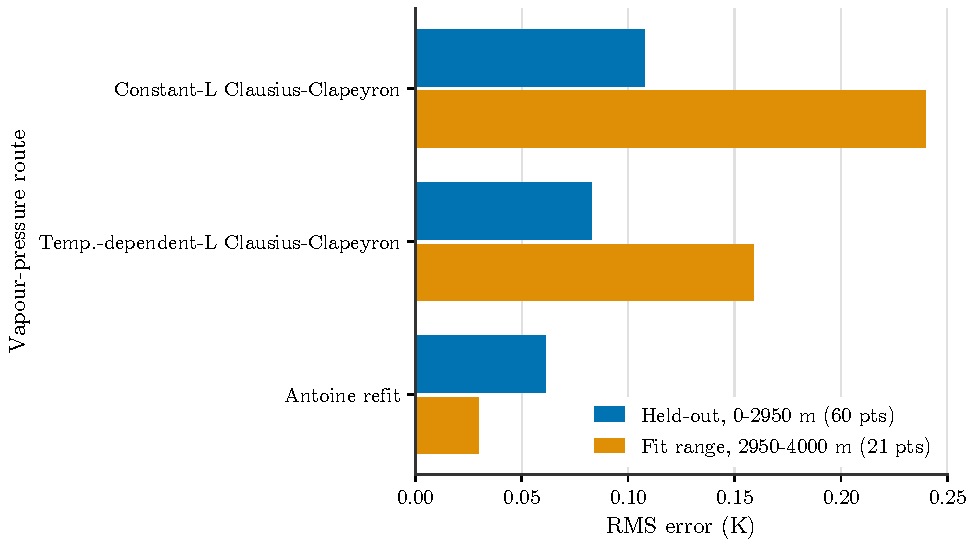
\includegraphics[width=\linewidth,height=0.45\textheight,keepaspectratio]{figures/fig2_v0.pdf}
  \caption{RMS error of three vapour-pressure routes against the IAPWS-IF97 saturation equation, not measured boiling points, split into held-out and Antoine fit-range points. Both Clausius--Clapeyron routes err more in the fit range; the Antoine refit is most accurate on both splits. Single deterministic runs, so no error bars.}
  \label{fig:rms}
\end{figure}

The sensitivity fit gives a different held-out result (Table~\ref{tab:antoine-sens}). Its held-out set is a different band, 353.15 to 373.15 K, and it covers all 81 grid points. Its held-out RMS is 0.092436\,K and its largest error is 0.132504\,K at sea level. The two Antoine rows in that table use different evaluation sets, so this document does not compare the sensitivity RMS with the Clausius--Clapeyron RMS of 0.082794\,K. An earlier draft and the reviewer read the sensitivity result as reversing the held-out ranking. That comparison is not like-for-like, because the Clausius--Clapeyron figures were computed on the 60-point held-out set. Whether the ranking holds under the alternative fit window was not tested on a common set, so the ranking is recorded as provisional.

\input{tables/tab_antoine_sens.tex}

The regression check against iteration 1 did not pass for Antoine. The iteration 1 in-sample grid maximum was 0.0042\,K, and this run gives 0.035756\,K. The constant-latent-heat and temperature-dependent routes reproduced their iteration 1 values to within 0.005\,K. The experiment therefore marks its Antoine interpretation as provisional. The 0.0042\,K value is not confirmed by this run. Its origin is not resolved here. One candidate explanation is the change of fit window, from 273.15 to 373.15 K in iteration 1 to 273.15 to 363.15 K in iteration 2. This is consistent with the iteration 1 fit, which reports an RMS residual of 0.055289\,K over its full range, but it is not tested. No later iteration re-ran the iteration 1 fit window.

\input{tables/tab_regression.tex}

The Clapeyron check gives the attribution test that the reviewer asked for. Table~\ref{tab:clapeyron} shows the residual of the Clapeyron relation under five treatments of the vapour. Applying the vapour compressibility removes the failure. The ideal-vapour residual of 1.6261\,\% falls to 0.0610\,\% once $Z_\mathrm{v}$ is applied. That tests the attribution, which iteration 1 had only stated. The two rows that carry the test are the independent-curve rows: the Antoine derivative residual of 0.9204\,\% passes the 1\,\% tolerance narrowly, and the IAPWS-95 derivative residual of 0.0625\,\% passes with room to spare. The Z$_\mathrm{v}$-corrected IF97 row is near zero by construction, because the pressure derivative, the latent heat and the vapour compressibility all come from the same IAPWS-IF97 equations. The artifact's overall verdict is ``holds, but largely an identity'', and this document uses the same wording.

\input{tables/tab_clapeyron.tex}

Two further checks support the reference. The Antoine refit on 273.15 to 363.15 K has an RMS residual of 0.000264 in $\log_{10}$ pressure and converged in 22 function evaluations. The table of gen\_art\_dataset\_1, cross-checked against the IAPWS-IF97 route at 100 m steps, differs from the reference by a maximum absolute value of 0.0625\,K and a mean difference of $-0.018143$\,K. Both numbers are consistency checks between two calculations, not measurements.

\subsection{Review after iteration 2}

The reviewer gave iteration 2 a review score of 3, not blocking. The reviewer recomputed the route errors, the sensitivity fit, the Clapeyron residuals and the regression values, and found that they matched their result files. The principal objections were these.
\begin{itemize}
\item \textbf{Scope (major).} After two iterations the accepted measured set is empty, and every result is a model-to-reference comparison. The record answers the neighbouring question, not the question asked.
\item \textbf{Methodology (major).} NOAA GHCN-Daily and the NIST steam-table PDF were not fetched. Iteration 2 searched the same candidate pool as iteration 1, and its dead-ends section said only ``not tried''.
\item \textbf{Evidence (major).} The statement that Antoine is the best route was carried into the result and the learned-so-far sections, although the sensitivity fit gives a different held-out figure. The reviewer asked that the ranking be presented as dependent on the fit window.
\item \textbf{Rigour (major).} The iteration 1 figure of 0.0042\,K did not reproduce. The reviewer asked for the iteration 1 fit window to be re-run with the iteration 2 grid code, and to report both figures.
\item \textbf{Rigour (major).} The held-out set covers 0 to 2,950 m, and the in-sample set covers 2,950 to 4,000 m. The altitudes the hypothesis is most concerned with therefore sit in the in-sample band, and the 4,000 m error comes only from the fit-range points.
\item \textbf{Novelty (major).} The positive claims have no published neighbour in the record. The reviewer asked for a scholarly search, with queries and a nearest result for each claim.
\item \textbf{Rigour (major).} The structural term is a difference between two formulas under the chosen reference, not an empirical outcome. Its 0.59\,K value versus the 0.5\,K target is a statement about the hypothesis's constant.
\item \textbf{Clarity (minor).} The Clapeyron headline should lead with the independent-curve residuals, not with the identity-check residual.
\item \textbf{Rigour (minor).} The 8 $\times$ 10$^{-10}$\,K brentq agreement should cite its file (\texttt{audit/rederive\_out.json}, with a maximum gap of $8.06 \times 10^{-10}$\,K).
\item \textbf{Clarity (minor).} The source of the reference table should carry its URL and access date. The volume discrepancy should be settled by checksums.
\end{itemize}

\subsection{Hypothesis update after iteration 2}

The update was a \emph{cover} move again, because the measured comparison is still the open part of the request. It recorded the following changes.
\begin{itemize}
\item The measured comparison is stated as untested in the claim itself. Zero verified measured records were found after two iterations.
\item The 0.5\,K structural-term target is no longer framed as an empirical miss. The 0.59\,K value at 4,000 m is described as a property of the two formulas under the chosen reference.
\item The Antoine ranking was removed from the claim. Its held-out advantage depends on the fit window, and the iteration 1 figure did not reproduce.
\item The variable-latent-heat claim was dropped, because it was tested and gave a 36\,\% reduction, not the more-than-half reduction claimed.
\item Measured-record acquisition became the main step, with named sources and a held-out set fixed before analysis.
\item The empirical altitude fit and the local pressure calibration remain untested candidates, since they need measured sites first.
\item Confidence in the hypothesis decreased. The 0.3\,K and 0.6\,K predictions are still unsupported by any measurement, and the 4,000 m structural term uses almost all of the 0.6\,K altitude-only budget.
\end{itemize}

The update considered four directions: cover the measured comparison, fix the Antoine fit window, deepen the reference screens, and declare the measured comparison untested. It chose to cover, because the reviewer had asked to stop adding reference screens until measured records were obtained. The Antoine fit-window fix was listed as a secondary item. It was not run, because no iteration followed.

\subsection{Dead ends in iteration 2}

\begin{itemize}
\item \textbf{Measured site records: still not obtained.} The search found no record meeting the measured-record criteria. The Forbes (1857) table is the only lead that could yield measured rows, and it was not transcribed. The hypothesis's central comparison, predicted against observed boiling temperature, has not been run.
\item \textbf{NOAA GHCN-Daily and the NIST steam-table PDF: not reached.} Both were on the planned list and neither was fetched in this iteration. The record therefore does not show that they lack measured boiling records. It shows only that they were not tried.
\item \textbf{Antoine as the best route: weakened, not confirmed.} On held-out points Antoine still has the lowest RMS, but the margin over temperature-dependent-latent-heat Clausius--Clapeyron is 0.021532\,K. The sensitivity fit gives a held-out RMS of 0.092436\,K on a different evaluation set. The regression against iteration 1 did not reproduce the 0.0042\,K value. The ranking is provisional.
\item \textbf{Held-out split and altitude band.} The held-out set does not overlap the altitudes of greatest interest, 2,950 to 4,000 m. The fit-range results cannot be treated as held-out evidence.
\item \textbf{Clapeyron attribution: tested, and it holds only with care.} The ideal-vapour residual falls once compressibility is applied, but the Z$_\mathrm{v}$-corrected IF97 residual is an identity. The independent-curve rows carry the test.
\item \textbf{Nearest published results: not searched.} The reviewer asked for a scholarly search for each positive claim. No such search was run in this iteration, so no neighbour is named beyond the standard references already in the record. The claims in this iteration are therefore not credited as novel.
\item \textbf{Log and volume discrepancy, iteration 1: not resolved.} The checksum comparison the reviewer asked for was not done.
\end{itemize}

\subsection{Result of iteration 2}

The measured comparison, which is the question the run was set, has still not been run. Iteration 2 added the test that will run it (gen\_art\_experiment\_3), and it added the first sources checked against the record's own standards (gen\_art\_dataset\_2). None of the sources yielded a measured record.

On the reference equations, the iteration 2 results change two statements from iteration 1. The held-out Antoine error is 0.061262\,K RMS, and the iteration 1 statement of 0.004\,K did not reproduce. The Clapeyron attribution to the vapour compressibility is now tested, and it holds to 0.0610\,\% after correction. The structural term and the two Clausius--Clapeyron routes reproduce their iteration 1 values.

\section{What the run learned and what is still open}

The run answered only part of the question. Its positive results are model-to-reference numbers, and the one number a reader is most likely to take as a finding, the 4,000 m structural term, is a property of the two formulas, not a test against measurements.

The run's evidence now runs in three layers, and only the first is about the question asked.
\begin{itemize}
\item \textbf{Measured comparison: not run.} No measured boiling record with station pressure and elevation has been verified. The accepted set is empty, and the predictions of 0.3\,K (station pressure) and 0.6\,K (altitude only) are untested.
\item \textbf{Structural term of the isothermal form: 0.332\,K at 3,000 m and 0.588\,K at 4,000 m.} The 4,000 m value exceeds the 0.5\,K structural target. The value is reproduced across two iterations and three artifacts. It describes the two formulas under the reference, not a measured residual.
\item \textbf{Vapour-pressure routes against the reference.} The refitted Antoine equation has the lowest held-out RMS (0.061262\,K), ahead of temperature-dependent-latent-heat Clausius--Clapeyron (0.082794\,K) and constant-latent-heat Clausius--Clapeyron (0.107780\,K). The constant-latent-heat route reaches 0.279825\,K at 4,000 m. The Antoine ranking is provisional, because it depends on the fit range and the iteration 1 value did not reproduce.
\item \textbf{Clapeyron relation.} It holds once vapour compressibility is applied. The independent-curve residuals carry the test, and the verdict is largely an identity.
\item \textbf{Reference table.} It is consistent with the two reference calculations to 0.0625\,K at 100 m steps. It is not measured.
\end{itemize}

Open items for any later iteration are these. The Forbes (1857) table needs transcription and site elevations. The NOAA and NIST sources the reviewer named need to be fetched, or their access failures recorded with the URL and status. If records are found, the predicted-minus-observed residuals for the held-out set need computing. The Antoine fit window needs re-running at 273.15 to 373.15 K, so that the 0.0042\,K figure is either reproduced or explained. The held-out set should also be defined over the altitude band that the hypothesis targets. The scholarly search for the nearest published result of each positive claim has not been run.

\subsection{Bookkeeping}

Table~\ref{tab:trajectory} gives the bookkeeping for both iterations. Each iteration's move, review score and evidence state are recorded as the run's trajectory log gives them. The ledger spend is cumulative, and it covers LLM, tool and container spend billed so far, but not compute-rental time.

\input{tables/tab_trajectory.tex}

\subsection{Artifacts and code}

Table~\ref{tab:artifacts} lists every artifact the run produced, with its iteration and its code folder. The artifacts themselves stay on the run's storage volume, and each artifact's output files are the source of the numbers in this report. The code is in the repository linked from the table.

\input{tables/tab_artifacts.tex}

\section*{References}

[1] W. Wagner and A. Pru\ss{}, ``The IAPWS Formulation 1995 for the Thermodynamic Properties of Ordinary Water Substance for General and Scientific Use,'' \emph{Journal of Physical and Chemical Reference Data}, vol.~31, no.~2, pp.~387--535, 2002. doi:10.1063/1.1461829.

\end{document}
